\documentclass[32pt,aspectratio=169]{beamer}

\usepackage[utf8]{inputenc} % Character encoding, choose your machine's default 
                              % encoding; latin1 or utf8. If you want it read by
                              % others choose latin1.
\pdfinfo{
   /Author (Bashar Dudin)
   /Title  (Transportation problems)
   /Subject (Networks and Flows on Graphs)
}

\usepackage{./Style/My_Beamer} % This is my Beamer style.
\usepackage{./Style/Mystyle} % This is my own defined commands

%----------------------------------------------------------------------------------------
%   TITLE PAGE
%----------------------------------------------------------------------------------------

\author[BD]{Bashar Dudin}

\institute[]{EPITA}
 
\title{Networks and Flows on Graphs} % 
\subtitle{Optimal Transportation Problems}

\begin{document}

\begin{frame}[plain]
\titlepage % Print the title page as the first slide
\end{frame}

\begin{frame}{What is it about?}
  We are given a set of $m$ origins $O$ and a set of $n$ destinations
  $D$. \pause Origins are valued by positive integer numbers
  corresponding to available goods while desinations are valued by
  positive integer numbers corresponding to demand. \pause \alert{We
    assume the total number of available goods is equal to the number
    of needed ones.}  \pause Going from an origin to a destination has
  a given cost. The cost of an arrow $a$ corresponding to such a
  ``path'' is a positive integer written $c(a)$. \pause
  \begin{halfshyblock}{Optimal transportation problem}
    Find a bipartite non-negatively (integer-)weighted digraph $G=(V, A)$
    linking vertices in $O$ to those of $D$ such that the total cost
    \begin{displaymath}
      c(G) = \sum_{a \in A}w(a)c(a)
    \end{displaymath}
    is minimal among all possible digraphs. 
  \end{halfshyblock}
\end{frame}

\begin{frame}{Conveniently modeling a transporation problem}
  The following table/matrix represents the costs of ``paths'' going
  from a set of origins $\{I, II, III, IV\}$ to a set of destinations
  numbered from $1$ to $6$. 
  \begin{figure}
    \begin{tabular}{l|c|c|c|c|c|c|r}
      & \textit{1} & \textit{2} & \textit{3} & \textit{4} & \textit{5} & \textit{6} & \cellcolor{blue!50}\textbf{Av.}\\
      \hline
      \textit{I} & \cellcolor{blue!25}12 & \cellcolor{blue!25}27 & \cellcolor{blue!25}61 & \cellcolor{blue!25}49 & \cellcolor{blue!25}83 & \cellcolor{blue!25}35 & \cellcolor{blue!50}18  \\
      \hline 
      \textit{II} & \cellcolor{blue!25}23 & \cellcolor{blue!25}39 & \cellcolor{blue!25}78 & \cellcolor{blue!25}28 & \cellcolor{blue!25}65 & \cellcolor{blue!25}42 & \cellcolor{blue!50}32  \\
      \hline
      \textit{III} & \cellcolor{blue!25}67 & \cellcolor{blue!25}56 & \cellcolor{blue!25}92 & \cellcolor{blue!25}24 & \cellcolor{blue!25}53 & \cellcolor{blue!25}54 & \cellcolor{blue!50}14  \\
      \hline
      \textit{IV} & \cellcolor{blue!25}71 & \cellcolor{blue!25}43 & \cellcolor{blue!25}91 & \cellcolor{blue!25}67 & \cellcolor{blue!25}40 & \cellcolor{blue!25}49 & \cellcolor{blue!50}9 \\
      \hline 
      \cellcolor{blue!50}\textbf{De.} & \cellcolor{blue!50}9 & \cellcolor{blue!50}11 & \cellcolor{blue!50}28 & \cellcolor{blue!50}6 & \cellcolor{blue!50}14 & \cellcolor{blue!50}5 & \cellcolor{blue!60}73 \\
  \end{tabular}
\end{figure}
\pause The violet colored $(i, j)$ coefficient represents the cost
$c_{ij}$ of the path going from $i$ to $j$. The darker cells
correspond to available goods and demand, the available number of
goods at a line $i$ is written $a_i$ and the number of needed goods at
a column $j$ is $b_j$. Notice that the total amount of available goods
is the same as the number of needed ones.
\end{frame}

\begin{frame}{Conveniently modeling a transporation problem}
  The following table/matrix represents the costs of ``paths'' going
  from a set of origins $\{I, II, III, IV\}$ to a set of destinations
  numbered from $1$ to $6$. 
  \begin{figure}
    \begin{tabular}{l|c|c|c|c|c|c|r}
      & \textit{1} & \textit{2} & \textit{3} & \textit{4} & \textit{5} & \textit{6} & \cellcolor{blue!50}\textbf{Av.}\\
      \hline
      \textit{I} & \cellcolor{blue!25}12 & \cellcolor{blue!25}27 & \cellcolor{blue!25}61 & \cellcolor{blue!25}49 & \cellcolor{blue!25}83 & \cellcolor{blue!25}35 & \cellcolor{blue!50}18  \\
      \hline 
      \textit{II} & \cellcolor{blue!25}23 & \cellcolor{blue!25}39 & \cellcolor{blue!25}78 & \cellcolor{blue!25}28 & \cellcolor{blue!25}65 & \cellcolor{blue!25}42 & \cellcolor{blue!50}32  \\
      \hline
      \textit{III} & \cellcolor{blue!25}67 & \cellcolor{blue!25}56 & \cellcolor{blue!25}92 & \cellcolor{blue!25}24 & \cellcolor{blue!25}53 & \cellcolor{blue!25}54 & \cellcolor{blue!50}14  \\
      \hline
      \textit{IV} & \cellcolor{blue!25}71 & \cellcolor{blue!25}43 & \cellcolor{blue!25}91 & \cellcolor{blue!25}67 & \cellcolor{blue!25}40 & \cellcolor{blue!25}49 & \cellcolor{blue!50}9 \\
      \hline 
      \cellcolor{blue!50}\textbf{De.} & \cellcolor{blue!50}9 & \cellcolor{blue!50}11 & \cellcolor{blue!50}28 & \cellcolor{blue!50}6 & \cellcolor{blue!50}14 & \cellcolor{blue!50}5 & \cellcolor{blue!60}73 \\
  \end{tabular}
\end{figure}
Solving the previous transportation problem is about finding a
matrix $(x_{ij})$ such that
\begin{displaymath}
  \sum_{j=1}^n x_{ij} = a_i\;\; , \quad \sum_{i=1}^m x_{ij} = b_j \quad \text{and the total cost} \quad
  c_{tot}\big((x_{ij})\big) = \sum_{i=1}^m\sum_{j=1}^n x_{ij} c_{ij} \quad \text{is minimal}
\end{displaymath}
\end{frame}

\begin{frame}{Needed hypothesis}
  The algorithm we shall be giving subsequently starts by giving an
  answer to our transportation problem not taking into account the
  cost; i.e. we look for a matrix $(x_{ij})$ only
  satisfying\footnote{In fact, the Balas-Hammer algorithm, studied
    hereby,``takes into account'' the cost function.}
  \begin{equation}
    \label{1}
    \tag{$\star$}
    \sum_{j=1}^n x_{ij} = a_i\;\; \quad \text{and} \quad \sum_{i=1}^m x_{ij} = b_j
  \end{equation}
  In order to be able to get a re-usable (optimizable if not optimal)
  answer we'll need it to be \emph{non-degenerate} ;
  \begin{alertblock}{Non-degeneracy}
    A matrix $(x_{ij})$ satisfying (\ref{1}) is called a \emph{basic
      solution} if it has $nm - (n+m-1)$ zeros.
  \end{alertblock}
  \begin{rem}
    It is not always the best idea to look for a basic solution! The
    point is that, when you have one, you're sure to be able to get a
    better one, if it's not the best.
  \end{rem}
\end{frame}

\begin{frame}{First stage : finding a basic solution}
  \begin{algorithm}[H]
    \caption{Balas-Hammer}
    \small{
      \begin{algorithmic}[1]
       \Statex
       
       \Require $M$ a maximal rank matrix of costs having size
       $m \times n$ and positive integer entries, a positive integer
       $a_i$ for each line $i$ and one $b_j$ for each column $j$ (sums
       of which along lines and columns are equal)

       \Ensure A solution for the transportation problem defined
       by $M$, $(a_i)$ and $(b_j)$
       \Statex

       \State for each line and each column, compute the difference
       between the smallest integer in the line or column and the one
       just bigger
       
       \State get the line or column corresponding to the maximum of all differences
 
       \State get the address $(i, j)$ of the minimum cost of the
       corresponding line or column

       \State give the highest possible weight $x_{ij}$ 
       
       \State erase the \emph{saturated} line $i$ or column $j$,
       obtained previously from $M$ (all corresponding weights are $0$
       except for $x_{ij}$) and modify the number of available and needed goods
       accordingly

       \State start again till $M$ is empty
       \State \Return the matrix $(x_{ij})$

     \end{algorithmic}
     }
    \end{algorithm}
\end{frame}

\begin{frame}{Balas-Hammer : Working out an example}
  \begin{columns}
    \begin{column}{.6\textwidth}
      Write $\Delta$ for the difference of the minimum of any line or
      column with the number just bigger, in the same line or column.
      
      \begin{overlayarea}{\textwidth}{.5\textheight}
        \vspace{.5cm}
        \small{
          \begin{tabular}{c|c|c|c|c|c|c|c|r}
            & \textit{1} & \textit{2} & \textit{3} & \textit{4} & \textit{5} & \textit{6} & \cellcolor{blue!50}\textbf{Av.} & \color{blue}$\Delta$\\
            \hline
            \textit{I} & \cellcolor{blue!25}12 & \cellcolor{blue!25}27 & \cellcolor{blue!25}61 & \cellcolor{blue!25}49 & \cellcolor{blue!25}83 & \cellcolor{blue!25}35 & \cellcolor{blue!50}18 & \color{blue}15 \\
            \hline 
            \textit{II} & \cellcolor{blue!25}23 & \cellcolor{blue!25}39 & \cellcolor{blue!25}78 & \cellcolor{blue!25}28 & \cellcolor{blue!25}65 & \cellcolor{blue!25}42 & \cellcolor{blue!50}32 & \color{blue}5 \\
            \hline
            \textit{III} & \cellcolor{blue!25}67 & \cellcolor{blue!25}56 & \cellcolor{blue!25}92 & \cellcolor{blue!25}24 & \cellcolor{blue!25}53 & \cellcolor{blue!25}54 & \cellcolor{blue!50}14 & \cellcolor{orange}\color{blue}29 \\
            \hline
            \textit{IV} & \cellcolor{blue!25}71 & \cellcolor{blue!25}43 & \cellcolor{blue!25}91 & \cellcolor{blue!25}67 & \cellcolor{blue!25}40 & \cellcolor{blue!25}49 & \cellcolor{blue!50}9 & \color{blue}3 \\
            \hline 
            \cellcolor{blue!50}\textbf{De.} & \cellcolor{blue!50}9 & \cellcolor{blue!50}11 & \cellcolor{blue!50}28 & \cellcolor{blue!50}6 & \cellcolor{blue!50}14 & \cellcolor{blue!50}5 & \cellcolor{blue!60}73 & \\            
            \cline{1-8}
            \color{blue}$\Delta$ & \color{blue}11 & \color{blue}12 & \color{blue}17 & \color{blue}4 & \color{blue}13 & \color{blue}7   
          \end{tabular}
        }
      \end{overlayarea}
    \end{column}
    \begin{column}{.4\textwidth}
      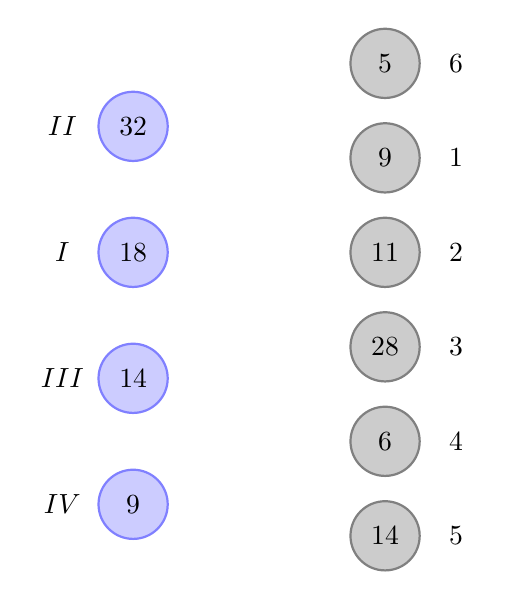
\begin{tikzpicture}
        [scale =.8, minimum width={width("28")+1.5em},
        origin/.style={circle,draw=blue!50,fill=blue!20,thick},
        destination/.style={circle,draw=black!50,fill=black!20,thick},
        arr/.style={->,>=stealth',semithick}]
        \node (6) at (5,9) [destination, label=0:$6$] {$5$};
        \node (1) at (5,7.5) [destination, label=0:$1$] {$9$};
        \node (2) at (5,6) [destination, label=0:$2$] {$11$};
        \node (3) at (5,4.5) [destination, label=0:$3$] {$28$};
        \node (4) at (5,3) [destination, label=0:$4$] {$6$};
        \node (5) at (5,1.5) [destination, label=0:$5$] {$14$};
        \node (II) at (1,8) [origin, label=180:$II$] {$32$};
        \node (I) at (1,6) [origin, label=180:$I$] {$18$};       
        \node (III) at (1,4) [origin, label=180:$III$] {$14$};
        \node (VI) at (1,2) [origin, label=180:$IV$] {$9$};
      \end{tikzpicture}
    \end{column}
  \end{columns}
\end{frame}

\begin{frame}{Balas-Hammer : Working out an example}
  \begin{columns}
    \begin{column}{.6\textwidth}
      The maximum of differences is $29$ at row $III$. The minimum of
      cost of row $III$ is $24$. It corresponds to the path from origin
      $III$ to destination $4$.

      \begin{overlayarea}{\textwidth}{.5\textheight}      
        \vspace{.45cm}
        \small{
          \begin{tabular}{c|c|c|c|c|c|c|c|r}
            & \textit{1} & \textit{2} & \textit{3} & \textit{4} & \textit{5} & \textit{6} & \cellcolor{blue!50}\textbf{Av.} & \color{blue}$\Delta$\\
            \hline
            \textit{I} & \cellcolor{blue!25}12 & \cellcolor{blue!25}27 & \cellcolor{blue!25}61 & \cellcolor{orange}49 & \cellcolor{blue!25}83 & \cellcolor{blue!25}35 & \cellcolor{blue!50}18 & \color{blue}15 \\
            \hline 
            \textit{II} & \cellcolor{blue!25}23 & \cellcolor{blue!25}39 & \cellcolor{blue!25}78 & \cellcolor{orange}28 & \cellcolor{blue!25}65 & \cellcolor{blue!25}42 & \cellcolor{blue!50}32 & \color{blue}5 \\
            \hline
            \cellcolor{orange}\textit{III} & \cellcolor{orange}67 & \cellcolor{orange}56 & \cellcolor{orange}92 & \cellcolor{orange}24 & \cellcolor{orange}53 & \cellcolor{orange}54 & \cellcolor{blue!50}14 & \cellcolor{orange}\color{blue}29 \\
            \hline
            \textit{IV} & \cellcolor{blue!25}71 & \cellcolor{blue!25}43 & \cellcolor{blue!25}91 & \cellcolor{orange}67 & \cellcolor{blue!25}40 & \cellcolor{blue!25}49 & \cellcolor{blue!50}9 & \color{blue}3 \\
            \hline 
            \cellcolor{blue!50}\textbf{De.} & \cellcolor{blue!50}9 & \cellcolor{blue!50}11 & \cellcolor{blue!50}28 & \cellcolor{blue!50}6 & \cellcolor{blue!50}14 & \cellcolor{blue!50}5 & \cellcolor{blue!60}73 & \\            
            \cline{1-8}
            \color{blue}$\Delta$ & \color{blue}11 & \color{blue}12 & \color{blue}17 & \color{blue}4 & \color{blue}13 & \color{blue}7   
          \end{tabular}
        }
      \end{overlayarea}
    \end{column}
    \begin{column}{.4\textwidth}
        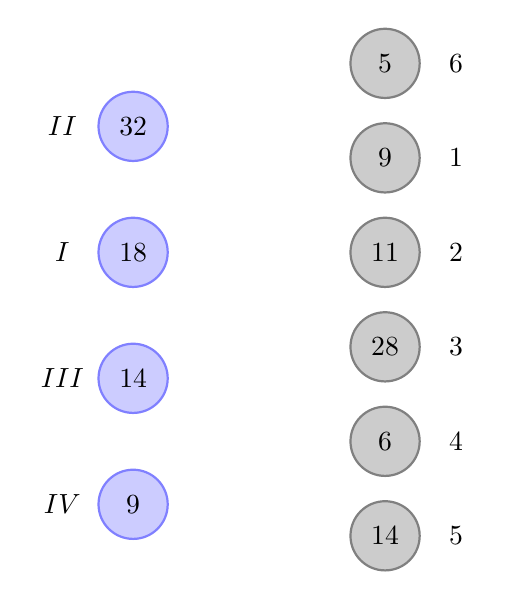
\begin{tikzpicture}
        [scale =.8, minimum width={width("28")+1.5em},
        origin/.style={circle,draw=blue!50,fill=blue!20,thick},
        destination/.style={circle,draw=black!50,fill=black!20,thick},
        arr/.style={->,>=stealth',semithick}]
        \node (6) at (5,9) [destination, label=0:$6$] {$5$};
        \node (1) at (5,7.5) [destination, label=0:$1$] {$9$};
        \node (2) at (5,6) [destination, label=0:$2$] {$11$};
        \node (3) at (5,4.5) [destination, label=0:$3$] {$28$};
        \node (4) at (5,3) [destination, label=0:$4$] {$6$};
        \node (5) at (5,1.5) [destination, label=0:$5$] {$14$};
        \node (II) at (1,8) [origin, label=180:$II$] {$32$};
        \node (I) at (1,6) [origin, label=180:$I$] {$18$};       
        \node (III) at (1,4) [origin, label=180:$III$] {$14$};
        \node (VI) at (1,2) [origin, label=180:$IV$] {$9$};
      \end{tikzpicture}
      \end{column}
    \end{columns}
\end{frame}

\begin{frame}{Balas-Hammer : Working out an example}
  \begin{columns}
    \begin{column}{.6\textwidth}
      There are $14$ available goods at origin $III$ and $6$ needed at
      destination $4$. We thus choose $x_{III,4} = 6$ and one can
      forget about column $4$.

      \begin{overlayarea}{\textwidth}{.5\textheight}      
        \vspace{.45cm}
        \small{
          \begin{tabular}{c|c|c|c|c|c|c|c|r}
            & \textit{1} & \textit{2} & \textit{3} & \textit{4} & \textit{5} & \textit{6} & \cellcolor{blue!50}\textbf{Av.} & \color{blue}$\Delta$\\
            \hline
            \textit{I} & \cellcolor{blue!25}12 & \cellcolor{blue!25}27 & \cellcolor{blue!25}61 & \cellcolor{orange}49 & \cellcolor{blue!25}83 & \cellcolor{blue!25}35 & \cellcolor{blue!50}18 & \color{blue}15 \\
            \hline 
            \textit{II} & \cellcolor{blue!25}23 & \cellcolor{blue!25}39 & \cellcolor{blue!25}78 & \cellcolor{orange}28 & \cellcolor{blue!25}65 & \cellcolor{blue!25}42 & \cellcolor{blue!50}32 & \color{blue}5 \\
            \hline
            \cellcolor{orange}\textit{III} & \cellcolor{orange}67 & \cellcolor{orange}56 & \cellcolor{orange}92 & \cellcolor{orange}24 & \cellcolor{orange}53 & \cellcolor{orange}54 & \cellcolor{blue!50}14 & \cellcolor{orange}\color{blue}29 \\
            \hline
            \textit{IV} & \cellcolor{blue!25}71 & \cellcolor{blue!25}43 & \cellcolor{blue!25}91 & \cellcolor{orange}67 & \cellcolor{blue!25}40 & \cellcolor{blue!25}49 & \cellcolor{blue!50}9 & \color{blue}3 \\
            \hline 
            \cellcolor{blue!50}\textbf{De.} & \cellcolor{blue!50}9 & \cellcolor{blue!50}11 & \cellcolor{blue!50}28 & \cellcolor{blue!50}6 & \cellcolor{blue!50}14 & \cellcolor{blue!50}5 & \cellcolor{blue!60}73 & \\            
            \cline{1-8}
            \color{blue}$\Delta$ & \color{blue}11 & \color{blue}12 & \color{blue}17 & \color{blue}4 & \color{blue}13 & \color{blue}7   
          \end{tabular}
        }
      \end{overlayarea}
    \end{column}
    \begin{column}{.4\textwidth}
        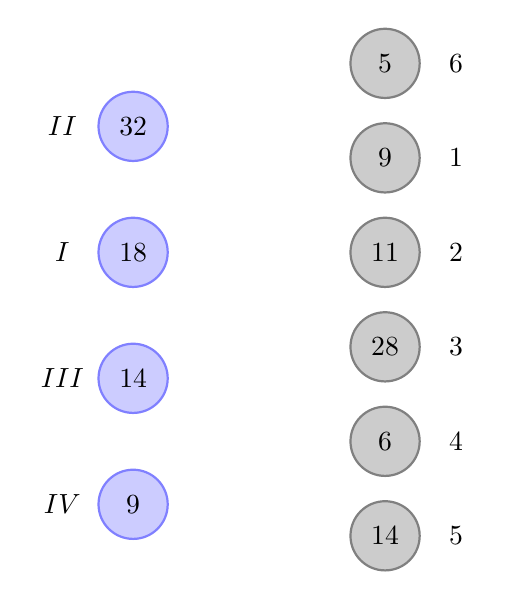
\begin{tikzpicture}
        [scale =.8, minimum width={width("28")+1.5em},
        origin/.style={circle,draw=blue!50,fill=blue!20,thick},
        destination/.style={circle,draw=black!50,fill=black!20,thick},
        arr/.style={->,>=stealth',semithick}]
        \node (6) at (5,9) [destination, label=0:$6$] {$5$};
        \node (1) at (5,7.5) [destination, label=0:$1$] {$9$};
        \node (2) at (5,6) [destination, label=0:$2$] {$11$};
        \node (3) at (5,4.5) [destination, label=0:$3$] {$28$};
        \node (4) at (5,3) [destination, label=0:$4$] {$6$};
        \node (5) at (5,1.5) [destination, label=0:$5$] {$14$};
        \node (II) at (1,8) [origin, label=180:$II$] {$32$};
        \node (I) at (1,6) [origin, label=180:$I$] {$18$};       
        \node (III) at (1,4) [origin, label=180:$III$] {$14$};
        \node (VI) at (1,2) [origin, label=180:$IV$] {$9$};
      \end{tikzpicture}

      \end{column}
    \end{columns}
\end{frame}


\begin{frame}{Balas-Hammer : Working out an example}
  \begin{columns}
    \begin{column}{.6\textwidth}
      There are $14$ available goods at origin $III$ and $6$ needed at
      destination $4$. We thus choose $x_{III,4} = 6$ and one can
      forget about column $4$.

      \begin{overlayarea}{\textwidth}{.5\textheight}      
        \vspace{.45cm}
        \small{
          \begin{tabular}{c|c|c|c|c|c|c|c|r}
            & \textit{1} & \textit{2} & \textit{3} & \textit{4} & \textit{5} & \textit{6} & \cellcolor{blue!50}\textbf{Av.} & \color{blue}$\Delta$\\
            \hline
            \textit{I} & \cellcolor{blue!25}12 & \cellcolor{blue!25}27 & \cellcolor{blue!25}61 & \cellcolor{orange}49 & \cellcolor{blue!25}83 & \cellcolor{blue!25}35 & \cellcolor{blue!50}18 & \color{blue}15 \\
            \hline 
            \textit{II} & \cellcolor{blue!25}23 & \cellcolor{blue!25}39 & \cellcolor{blue!25}78 & \cellcolor{orange}28 & \cellcolor{blue!25}65 & \cellcolor{blue!25}42 & \cellcolor{blue!50}32 & \color{blue}5 \\
            \hline
            \cellcolor{orange}\textit{III} & \cellcolor{orange}67 & \cellcolor{orange}56 & \cellcolor{orange}92 & \cellcolor{orange}24 & \cellcolor{orange}53 & \cellcolor{orange}54 & \cellcolor{blue!50}14 & \cellcolor{orange}\color{blue}29 \\
            \hline
            \textit{IV} & \cellcolor{blue!25}71 & \cellcolor{blue!25}43 & \cellcolor{blue!25}91 & \cellcolor{orange}67 & \cellcolor{blue!25}40 & \cellcolor{blue!25}49 & \cellcolor{blue!50}9 & \color{blue}3 \\
            \hline 
            \cellcolor{blue!50}\textbf{De.} & \cellcolor{blue!50}9 & \cellcolor{blue!50}11 & \cellcolor{blue!50}28 & \cellcolor{blue!50}6 & \cellcolor{blue!50}14 & \cellcolor{blue!50}5 & \cellcolor{blue!60}73 & \\            
            \cline{1-8}
            \color{blue}$\Delta$ & \color{blue}11 & \color{blue}12 & \color{blue}17 & \color{blue}4 & \color{blue}13 & \color{blue}7   
          \end{tabular}
        }
        \begin{tikzpicture}[baseline, overlay]
          \draw[red, ultra thick] (-3.7, -2) -- (-3.7, 2);
        \end{tikzpicture}
      \end{overlayarea}
    \end{column}
    \begin{column}{.4\textwidth}
        \begin{tikzpicture}
        [scale =.8, minimum width={width("28")+1.5em},
        origin/.style={circle,draw=blue!50,fill=blue!20,thick},
        destination/.style={circle,draw=black!50,fill=black!20,thick},
        arr/.style={->,>=stealth',semithick}]
        \node (6) at (5,9) [destination, label=0:$6$] {$5$};
        \node (1) at (5,7.5) [destination, label=0:$1$] {$9$};
        \node (2) at (5,6) [destination, label=0:$2$] {$11$};
        \node (3) at (5,4.5) [destination, label=0:$3$] {$28$};
        \node (4) at (5,3) [destination, label=0:$4$] {$6$};
        \node (5) at (5,1.5) [destination, label=0:$5$] {$14$};
        \node (II) at (1,8) [origin, label=180:$II$] {$32$};
        \node (I) at (1,6) [origin, label=180:$I$] {$18$};       
        \node (III) at (1,4) [origin, label=180:$III$] {$14$}
           edge[arr] node[above,red] {$6$} (4);        
        \node (VI) at (1,2) [origin, label=180:$IV$] {$9$};
      \end{tikzpicture}
      \end{column}
    \end{columns}
\end{frame}

\begin{frame}{Balas-Hammer : Working out an example}
  \begin{columns}
    \begin{column}{.6\textwidth}
      We thus find ourselves with a smaller matrix. In this new matrix
      cost doesn't change but there are less available goods at origin
      $III$ because $6$ went to fill the need at destination $4$.

      \begin{overlayarea}{\textwidth}{.5\textheight}      
        \vspace{.22cm}
        \small{
          \begin{tabular}{c|c|c|c|c|c|c|c|r}
            & \textit{1} & \textit{2} & \textit{3} & \textit{5} & \textit{6} & \cellcolor{blue!50}\textbf{Av.} \\
            \hline
            \textit{I} & \cellcolor{blue!25}12 & \cellcolor{blue!25}27 & \cellcolor{blue!25}61 & \cellcolor{blue!25}83 & \cellcolor{blue!25}35 & \cellcolor{blue!50}18 \\
            \hline 
            \textit{II} & \cellcolor{blue!25}23 & \cellcolor{blue!25}39 & \cellcolor{blue!25}78 &  \cellcolor{blue!25}65 & \cellcolor{blue!25}42 & \cellcolor{blue!50}32 \\
            \hline
            \textit{III} & \cellcolor{blue!25}67 & \cellcolor{blue!25}56 & \cellcolor{blue!25}92 & \cellcolor{blue!25}53 & \cellcolor{blue!25}54 & \cellcolor{blue!50}8 \\
            \hline
            \textit{IV} & \cellcolor{blue!25}71 & \cellcolor{blue!25}43 & \cellcolor{blue!25}91 & \cellcolor{blue!25}40 & \cellcolor{blue!25}49 & \cellcolor{blue!50}9 \\
            \hline 
            \cellcolor{blue!50}\textbf{De.} & \cellcolor{blue!50}9 & \cellcolor{blue!50}11 & \cellcolor{blue!50}28 & \cellcolor{blue!50}14 & \cellcolor{blue!50}5 & \cellcolor{blue!60}67  \\            
          \end{tabular}
        }
      \end{overlayarea}
    \end{column}
    \begin{column}{.4\textwidth}
        \begin{tikzpicture}
        [scale =.8, minimum width={width("28")+1.5em},
        origin/.style={circle,draw=blue!50,fill=blue!20,thick},
        destination/.style={circle,draw=black!50,fill=black!20,thick},
        arr/.style={->,>=stealth',semithick}]
        \node (6) at (5,9) [destination, label=0:$6$] {$5$};
        \node (1) at (5,7.5) [destination, label=0:$1$] {$9$};
        \node (2) at (5,6) [destination, label=0:$2$] {$11$};
        \node (3) at (5,4.5) [destination, label=0:$3$] {$28$};
        \node (4) at (5,3) [destination, label=0:$4$] {$6$};
        \node (5) at (5,1.5) [destination, label=0:$5$] {$14$};
        \node (II) at (1,8) [origin, label=180:$II$] {$32$};
        \node (I) at (1,6) [origin, label=180:$I$] {$18$};       
        \node (III) at (1,4) [origin, label=180:$III$] {$14$}
           edge[arr] node[above,red] {$6$} (4);        
        \node (VI) at (1,2) [origin, label=180:$IV$] {$9$};
      \end{tikzpicture}
      \end{column}
    \end{columns}
\end{frame}

\begin{frame}{Balas-Hammer : Working out an example}
  \begin{columns}
    \begin{column}{.6\textwidth}
      \vfill
      
      Let us run one more step towards building a basic solution to
      our transportation problem.
      \vspace{1.3\baselineskip}

      \begin{overlayarea}{\textwidth}{.5\textheight}      
        \vspace{.22cm}
        \small{
          \begin{tabular}{c|c|c|c|c|c|c|r}
            & \textit{1} & \textit{2} & \textit{3} & \textit{5} & \textit{6} & \cellcolor{blue!50}\textbf{Av.} & \color{blue}$\Delta$ \\
            \hline
            \textit{I} & \cellcolor{blue!25}12 & \cellcolor{blue!25}27 & \cellcolor{blue!25}61 & \cellcolor{blue!25}83 & \cellcolor{blue!25}35 & \cellcolor{blue!50}18 & \color{blue}15 \\
            \hline 
            \textit{II} & \cellcolor{blue!25}23 & \cellcolor{blue!25}39 & \cellcolor{blue!25}78 &  \cellcolor{blue!25}65 & \cellcolor{blue!25}42 & \cellcolor{blue!50}32 & \color{blue}16\\
            \hline
            \textit{III} & \cellcolor{blue!25}67 & \cellcolor{blue!25}56 & \cellcolor{blue!25}92 & \cellcolor{blue!25}53 & \cellcolor{blue!25}54 & \cellcolor{blue!50}8 & \color{blue}1\\
            \hline
            \textit{IV} & \cellcolor{blue!25}71 & \cellcolor{blue!25}43 & \cellcolor{blue!25}91 & \cellcolor{blue!25}40 & \cellcolor{blue!25}49 & \cellcolor{blue!50}9 & \color{blue}3\\
            \hline 
            \cellcolor{blue!50}\textbf{De.} & \cellcolor{blue!50}9 & \cellcolor{blue!50}11 & \cellcolor{blue!50}28 & \cellcolor{blue!50}14 & \cellcolor{blue!50}5 & \cellcolor{blue!60}67  \\
            \cline{1-7}
            \color{blue}$\Delta$ & \color{blue}11 & \color{blue}12 & \color{blue}17 & \color{blue}13 & \color{blue}7
          \end{tabular}
        }
      \end{overlayarea}
    \end{column}
    \begin{column}{.4\textwidth}
        \begin{tikzpicture}
        [scale =.8, minimum width={width("28")+1.5em},
        origin/.style={circle,draw=blue!50,fill=blue!20,thick},
        destination/.style={circle,draw=black!50,fill=black!20,thick},
        arr/.style={->,>=stealth',semithick}]
        \node (6) at (5,9) [destination, label=0:$6$] {$5$};
        \node (1) at (5,7.5) [destination, label=0:$1$] {$9$};
        \node (2) at (5,6) [destination, label=0:$2$] {$11$};
        \node (3) at (5,4.5) [destination, label=0:$3$] {$28$};
        \node (4) at (5,3) [destination, label=0:$4$] {$6$};
        \node (5) at (5,1.5) [destination, label=0:$5$] {$14$};
        \node (II) at (1,8) [origin, label=180:$II$] {$32$};
        \node (I) at (1,6) [origin, label=180:$I$] {$18$};       
        \node (III) at (1,4) [origin, label=180:$III$] {$14$}
           edge[arr] node[above,red] {$6$} (4);        
        \node (VI) at (1,2) [origin, label=180:$IV$] {$9$};
      \end{tikzpicture}
      \end{column}
    \end{columns}
\end{frame}

\begin{frame}{Balas-Hammer : Working out an example}
  \begin{columns}
    \begin{column}{.6\textwidth}
      \vfill
      
      Let us run one more step towards building a basic solution to
      our transportation problem.
      \vspace{1.3\baselineskip}

      \begin{overlayarea}{\textwidth}{.5\textheight}      
        \vspace{.22cm}
        \small{
          \begin{tabular}{c|c|c|c|c|c|c|r}
            & \textit{1} & \textit{2} & \cellcolor{orange}\textit{3} & \textit{5} & \textit{6} & \cellcolor{blue!50}\textbf{Av.} & \color{blue}$\Delta$ \\
            \hline
            \textit{I} & \cellcolor{orange}12 & \cellcolor{orange}27 & \cellcolor{orange}61 & \cellcolor{orange}83 & \cellcolor{orange}35 & \cellcolor{blue!50}18 & \color{blue}15 \\
            \hline 
            \textit{II} & \cellcolor{blue!25}23 & \cellcolor{blue!25}39 & \cellcolor{orange}78 &  \cellcolor{blue!25}65 & \cellcolor{blue!25}42 & \cellcolor{blue!50}32 & \color{blue}16\\
            \hline
            \textit{III} & \cellcolor{blue!25}67 & \cellcolor{blue!25}56 & \cellcolor{orange}92 & \cellcolor{blue!25}53 & \cellcolor{blue!25}54 & \cellcolor{blue!50}8 & \color{blue}1\\
            \hline
            \textit{IV} & \cellcolor{blue!25}71 & \cellcolor{blue!25}43 & \cellcolor{orange}91 & \cellcolor{blue!25}40 & \cellcolor{blue!25}49 & \cellcolor{blue!50}9 & \color{blue}3\\
            \hline 
            \cellcolor{blue!50}\textbf{De.} & \cellcolor{blue!50}9 & \cellcolor{blue!50}11 & \cellcolor{blue!50}28 & \cellcolor{blue!50}14 & \cellcolor{blue!50}5 & \cellcolor{blue!60}67  \\
            \cline{1-7}
            \color{blue}$\Delta$ & \color{blue}11 & \color{blue}12 & \cellcolor{orange}\color{blue}17 & \color{blue}13 & \color{blue}7
          \end{tabular}
        }
        
      \end{overlayarea}
    \end{column}
    \begin{column}{.4\textwidth}
        \begin{tikzpicture}
        [scale =.8, minimum width={width("28")+1.5em},
        origin/.style={circle,draw=blue!50,fill=blue!20,thick},
        destination/.style={circle,draw=black!50,fill=black!20,thick},
        arr/.style={->,>=stealth',semithick}]
        \node (6) at (5,9) [destination, label=0:$6$] {$5$};
        \node (1) at (5,7.5) [destination, label=0:$1$] {$9$};
        \node (2) at (5,6) [destination, label=0:$2$] {$11$};
        \node (3) at (5,4.5) [destination, label=0:$3$] {$28$};
        \node (4) at (5,3) [destination, label=0:$4$] {$6$};
        \node (5) at (5,1.5) [destination, label=0:$5$] {$14$};
        \node (II) at (1,8) [origin, label=180:$II$] {$32$};
        \node (I) at (1,6) [origin, label=180:$I$] {$18$};       
        \node (III) at (1,4) [origin, label=180:$III$] {$14$}
           edge[arr] node[above,red] {$6$} (4);        
        \node (VI) at (1,2) [origin, label=180:$IV$] {$9$};
      \end{tikzpicture}
      \end{column}
    \end{columns}
\end{frame}

\begin{frame}{Balas-Hammer : Working out an example}
  \begin{columns}
    \begin{column}{.6\textwidth}
      \vfill
      
      Let us run one more step towards building a basic solution to
      our transportation problem.
      \vspace{1.3\baselineskip}

      \begin{overlayarea}{\textwidth}{.5\textheight}      
        \vspace{.22cm}
        \small{
          \begin{tabular}{c|c|c|c|c|c|c|r}
            & \textit{1} & \textit{2} & \cellcolor{orange}\textit{3} & \textit{5} & \textit{6} & \cellcolor{blue!50}\textbf{Av.} & \color{blue}$\Delta$ \\
            \hline
            \textit{I} & \cellcolor{orange}12 & \cellcolor{orange}27 & \cellcolor{orange}61 & \cellcolor{orange}83 & \cellcolor{orange}35 & \cellcolor{blue!50}18 & \color{blue}15 \\
            \hline 
            \textit{II} & \cellcolor{blue!25}23 & \cellcolor{blue!25}39 & \cellcolor{orange}78 &  \cellcolor{blue!25}65 & \cellcolor{blue!25}42 & \cellcolor{blue!50}32 & \color{blue}16\\
            \hline
            \textit{III} & \cellcolor{blue!25}67 & \cellcolor{blue!25}56 & \cellcolor{orange}92 & \cellcolor{blue!25}53 & \cellcolor{blue!25}54 & \cellcolor{blue!50}8 & \color{blue}1\\
            \hline
            \textit{IV} & \cellcolor{blue!25}71 & \cellcolor{blue!25}43 & \cellcolor{orange}91 & \cellcolor{blue!25}40 & \cellcolor{blue!25}49 & \cellcolor{blue!50}9 & \color{blue}3\\
            \hline 
            \cellcolor{blue!50}\textbf{De.} & \cellcolor{blue!50}9 & \cellcolor{blue!50}11 & \cellcolor{blue!50}28 & \cellcolor{blue!50}14 & \cellcolor{blue!50}5 & \cellcolor{blue!60}67  \\
            \cline{1-7}
            \color{blue}$\Delta$ & \color{blue}11 & \color{blue}12 & \cellcolor{orange}\color{blue}17 & \color{blue}13 & \color{blue}7
          \end{tabular}
        }
        \begin{tikzpicture}[baseline, overlay]
          \draw[red, ultra thick] (-6.7, 1.1) -- (0, 1.1);
        \end{tikzpicture}
      \end{overlayarea}
    \end{column}
    \begin{column}{.4\textwidth}
      \begin{tikzpicture}
        [scale =.8, minimum width={width("28")+1.5em},
        origin/.style={circle,draw=blue!50,fill=blue!20,thick},
        destination/.style={circle,draw=black!50,fill=black!20,thick},
        arr/.style={->,>=stealth',semithick}]
        \node (6) at (5,9) [destination, label=0:$6$] {$5$};
        \node (1) at (5,7.5) [destination, label=0:$1$] {$9$};
        \node (2) at (5,6) [destination, label=0:$2$] {$11$};
        \node (3) at (5,4.5) [destination, label=0:$3$] {$28$};
        \node (4) at (5,3) [destination, label=0:$4$] {$6$};
        \node (5) at (5,1.5) [destination, label=0:$5$] {$14$};
        \node (II) at (1,8) [origin, label=180:$II$] {$32$};
        \node (I) at (1,6) [origin, label=180:$I$] {$18$}
           edge[arr] node[above,pos=0.3, red] {$18$} (3);       
        \node (III) at (1,4) [origin, label=180:$III$] {$14$}
           edge[arr] node[above,red] {$6$} (4);        
        \node (VI) at (1,2) [origin, label=180:$IV$] {$9$};
      \end{tikzpicture}
      \end{column}
    \end{columns}
\end{frame}

\begin{frame}{Balas-Hammer : Working out an example}
  \begin{columns}
    \begin{column}{.6\textwidth}
      \vfill
      
      Let us run one more step towards building a basic solution to
      our transportation problem.
      \vspace{1.3\baselineskip}

      \begin{overlayarea}{\textwidth}{.5\textheight}      
        \vspace{.22cm}
        \small{
          \begin{tabular}{c|c|c|c|c|c|c|r}
            & \textit{1} & \textit{2} & \textit{3} & \textit{5} & \textit{6} & \cellcolor{blue!50}\textbf{Av.}  \\
            \hline
            \textit{II} & \cellcolor{blue!25}23 & \cellcolor{blue!25}39 & \cellcolor{blue!25}78 &  \cellcolor{blue!25}65 & \cellcolor{blue!25}42 & \cellcolor{blue!50}32 \\
            \hline
            \textit{III} & \cellcolor{blue!25}67 & \cellcolor{blue!25}56 & \cellcolor{blue!25}92 & \cellcolor{blue!25}53 & \cellcolor{blue!25}54 & \cellcolor{blue!50}8 \\
            \hline
            \textit{IV} & \cellcolor{blue!25}71 & \cellcolor{blue!25}43 & \cellcolor{blue!25}91 & \cellcolor{blue!25}40 & \cellcolor{blue!25}49 & \cellcolor{blue!50}9 \\
            \hline 
            \cellcolor{blue!50}\textbf{De.} & \cellcolor{blue!50}9 & \cellcolor{blue!50}11 & \cellcolor{blue!50}10 & \cellcolor{blue!50}14 & \cellcolor{blue!50}5 & \cellcolor{blue!60}49  \\
          \end{tabular}
        }
      \end{overlayarea}
    \end{column}
    \begin{column}{.4\textwidth}
      \begin{tikzpicture}
        [scale =.8, minimum width={width("28")+1.5em},
        origin/.style={circle,draw=blue!50,fill=blue!20,thick},
        destination/.style={circle,draw=black!50,fill=black!20,thick},
        arr/.style={->,>=stealth',semithick}]
        \node (6) at (5,9) [destination, label=0:$6$] {$5$};
        \node (1) at (5,7.5) [destination, label=0:$1$] {$9$};
        \node (2) at (5,6) [destination, label=0:$2$] {$11$};
        \node (3) at (5,4.5) [destination, label=0:$3$] {$28$};
        \node (4) at (5,3) [destination, label=0:$4$] {$6$};
        \node (5) at (5,1.5) [destination, label=0:$5$] {$14$};
        \node (II) at (1,8) [origin, label=180:$II$] {$32$};
        \node (I) at (1,6) [origin, label=180:$I$] {$18$}
           edge[arr] node[above,pos=0.3, red] {$18$} (3);       
        \node (III) at (1,4) [origin, label=180:$III$] {$14$}
           edge[arr] node[above,red] {$6$} (4);        
        \node (VI) at (1,2) [origin, label=180:$IV$] {$9$};
      \end{tikzpicture}
      \end{column}
    \end{columns}
\end{frame}

\begin{frame}{Tree Structure Underlying a Basic Solution}
  \begin{columns}
    \begin{column}{.6\textwidth}
      Running Balas-Hammer algorithm till the end we get the solution
      on the right. 

      \vspace{.5\baselineskip}
      Notice now that the condition to be a \emph{basic}
      solution means that you get a graph having $m + n$ vertices ($m$
      origins and $n$ destinations) with $m+n-1$ arrows; it is thus
      a \alert{tree}! \\
      In the case at hand we got $4+6-1 = 9$ arrows
      and one can check by looking at the graph on the right that it
      is a tree.
      
      \vspace{.5\baselineskip}       
      We are going to use this tree structure for the second step of
      our algorithm: optimizing the transportation program we have.
    \end{column}
    \begin{column}{.4\textwidth}
      \begin{tikzpicture}
        [scale =.8, minimum width={width("28")+1.5em},
        origin/.style={circle,draw=blue!50,fill=blue!20,thick},
        destination/.style={circle,draw=black!50,fill=black!20,thick},
        arr/.style={->,>=stealth',semithick}]
        \node (6) at (5,9) [destination, label=0:$6$] {$5$};
        \node (1) at (5,7.5) [destination, label=0:$1$] {$9$};
        \node (2) at (5,6) [destination, label=0:$2$] {$11$};
        \node (3) at (5,4.5) [destination, label=0:$3$] {$28$};
        \node (4) at (5,3) [destination, label=0:$4$] {$6$};
        \node (5) at (5,1.5) [destination, label=0:$5$] {$14$};
        \node (II) at (1,8) [origin, label=180:$II$] {$32$}
        edge[arr] node[above,pos=0.3, red] {$5$} (6)
           edge[arr] node[above, red] {$9$} (1)
           edge[arr] node[above,pos=0.6, red] {$11$} (2)
           edge[arr] node[above,pos=0.6, red] {$7$} (3);
        \node (I) at (1,6) [origin, label=180:$I$] {$18$}
           edge[arr] node[above,pos=0.3, red] {$18$} (3);       
        \node (III) at (1,4) [origin, label=180:$III$] {$14$}
           edge[arr] node[above,pos=0.4, red] {$3$} (3)
           edge[arr] node[above,red] {$6$} (4)
           edge[arr] node[above,pos=0.6,red] {$5$} (5);        
        \node (VI) at (1,2) [origin, label=180:$IV$] {$9$}
        edge[arr] node[above,pos=0.4, red] {$9$} (5);
\end{tikzpicture}
    \end{column}
  \end{columns}
\end{frame}

\begin{frame}{How to look for a better solution ?}
  \begin{columns}
   \begin{column}{.6\textwidth}
     \begin{overlayarea}{\textwidth}{.35\textheight}
       \begin{onlyenv}<1>
       We've got a basic solution, i.e. a matrix $(x_{ij})_{i,j}$ satisfying 
       \vskip-1em
       \begin{equation}
         \label{2}
         \tag{$\star$}
         \sum_{j=1}^n x_{ij} = a_i\;\; \quad \text{and} \quad \sum_{i=1}^m x_{ij} = b_j
       \end{equation}
       \vskip-.5em
       where $a_i$ is the number of goods available at $i$ and $b_j$ is
       the number of ones needed at $j$. 
     \end{onlyenv}
     \begin{onlyenv}<2>
       \vspace{\baselineskip}
       In order to understand how to
       look for a better one, let us start by reorganizing our data.
       Below is the matrix $(x_{ij})_{i, j}$ and on the write is the
       tree representing this solution with costs along arrows. 
     \end{onlyenv}
   \end{overlayarea}
   \begin{figure}
    \begin{tabular}{l|c|c|c|c|c|c|}
      & \cellcolor{red!20}{\textit{1}} & \cellcolor{red!20}{\textit{2}} & \cellcolor{red!20}{\textit{3}} & 
      \cellcolor{red!20}{\textit{4}} & \cellcolor{red!20}{\textit{5}} & \cellcolor{red!20}{\textit{6}} \\
      \hline
      \cellcolor{red!20}{\textit{I}} &  &  & 18 &  &  &   \\
      \hline 
      \cellcolor{red!20}{\textit{II}} & 9  & 11  & 7 &  &  & 5 \\
      \hline
      \cellcolor{red!20}{\textit{III}} &  &  & 3 & 6 & 5 & \\
      \hline
      \cellcolor{red!20}{\textit{IV}} &  &  &  &  & 9 &  \\
      \hline 
  \end{tabular}
\end{figure}
 \end{column}
 \begin{column}{.4\textwidth}
   \begin{tikzpicture}
     [
     scale =.8, minimum width={width("28")+1.5em},
     origin/.style={circle,draw=blue!50,fill=blue!20,thick},
     destination/.style={circle,draw=black!50,fill=black!20,thick},
     arr/.style={->,>=stealth',semithick}
     ]
     \node (6) at (5,9) [destination, label=0:$6$] {};
     \node (1) at (5,7.5) [destination, label=0:$1$] {};
     \node (2) at (5,6) [destination, label=0:$2$] {};
     \node (3) at (5,4.5) [destination, label=0:$3$] {};
     \node (4) at (5,3) [destination, label=0:$4$] {};
     \node (5) at (5,1.5) [destination, label=0:$5$] {};
     \node (II) at (1,8) [origin, label=180:$II$] {}
     edge[arr] node[above,pos=0.3, red] {$42$} (6)
     edge[arr] node[above, red] {$23$} (1)
     edge[arr] node[above,pos=0.6, red] {$39$} (2)
     edge[arr] node[above,pos=0.6, red] {$78$} (3);
     \node (I) at (1,6) [origin, label=180:$I$] {}
     edge[arr] node[above,pos=0.3, red] {$61$} (3);       
     \node (III) at (1,4) [origin, label=180:$III$] {}
     edge[arr] node[above,pos=0.4, red] {$92$} (3)
     edge[arr] node[above,red] {$24$} (4)
     edge[arr] node[above,pos=0.6,red] {$53$} (5);        
     \node (VI) at (1,2) [origin, label=180:$IV$] {}
     edge[arr] node[above,pos=0.4, red] {$40$} (5);
   \end{tikzpicture}
 \end{column}
\end{columns}
\end{frame}

\begin{frame}
  \frametitle{How to look for a better solution ?}
  \begin{columns}
   \begin{column}{.6\textwidth}
     \begin{overlayarea}{\textwidth}{.35\textheight}
       \begin{onlyenv}<1> 
         Assume we want to send a unit of goods along the unused path
         $(I, 1)$. This means we're adding $1$ to the $(I, 1)$
         coefficient of our matrix. For the final result to stay a
         solution to our transportation problem, we're forced to make
         at least $3$ other changes to our matrix.
     \end{onlyenv}
     \begin{onlyenv}<2> 
       These changes correspond to going around the green cycle in the
       graph on the right. Adding $+1$ to the path $(I, 1)$, taking
       $1$ out of the route along $(II, 1)$, adding it up to the route
       along $(II, 3)$ and then taking $1$ from the path $(I, 3)$.
     \end{onlyenv}
     \begin{onlyenv}<3> 
       
       Looking for a different solution is about looking for cycles in
       the tree on the right. For such a solution to be a
       \emph{better} solution, the \emph{marginal cost} along this
       cycle has to be negative. In our case
       $+ 12 - 23 + 78 - 61 = 6$, if we tried going through $(I, 1)$
       it would only get more expensive.
     \end{onlyenv}
   \end{overlayarea}
   \begin{figure}
    \begin{tabular}{l|c|c|c|c|c|c|}
      & \cellcolor{red!20}{\textit{1}} & \cellcolor{red!20}{\textit{2}} & \cellcolor{red!20}{\textit{3}} & 
      \cellcolor{red!20}{\textit{4}} & \cellcolor{red!20}{\textit{5}} & \cellcolor{red!20}{\textit{6}} \\
      \hline
      \cellcolor{red!20}{\textit{I}} & \color{green!50!black}{+1} &  & 18  \color{green!50!black}{-1} &  &  &   \\
      \hline 
      \cellcolor{red!20}{\textit{II}} & 9 \color{green!50!black}{-1}  & 11  & 7 \color{green!50!black}{+1} &  &  & 5 \\
      \hline
      \cellcolor{red!20}{\textit{III}} &  &  & 3 & 6 & 5 & \\
      \hline
      \cellcolor{red!20}{\textit{IV}} &  &  &  &  & 9 &  \\
      \hline 
  \end{tabular}
\end{figure}
 \end{column}
 \begin{column}{.4\textwidth}
   \begin{overlayarea}{\textwidth}{.78\textheight}
     \begin{onlyenv}<1>
       \begin{tikzpicture}
         [
         scale =.8, minimum width={width("28")+1.5em},
         origin/.style={circle,draw=blue!50,fill=blue!20,thick},
         destination/.style={circle,draw=black!50,fill=black!20,thick},
         arr/.style={->,>=stealth',semithick}
         ]
         \node (6) at (5,9) [destination, label=0:$6$] {};
         \node (1) at (5,7.5) [destination, label=0:$1$] {};
         \node (2) at (5,6) [destination, label=0:$2$] {};
         \node (3) at (5,4.5) [destination, label=0:$3$] {};
         \node (4) at (5,3) [destination, label=0:$4$] {};
         \node (5) at (5,1.5) [destination, label=0:$5$] {};
         \node (II) at (1,8) [origin, label=180:$II$] {}
         edge[arr] node[above,pos=0.3, red] {$42$} (6)
         edge[arr] node[above, red] {$23$} (1)
         edge[arr] node[above,pos=0.6, red] {$39$} (2)
         edge[arr] node[above,pos=0.6, red] {$78$} (3);
         \node (I) at (1,6) [origin, label=180:$I$] {}
         edge[arr] node[above,pos=0.3, red] {$61$} (3);       
         \node (III) at (1,4) [origin, label=180:$III$] {}
         edge[arr] node[above,pos=0.4, red] {$92$} (3)
         edge[arr] node[above,red] {$24$} (4)
         edge[arr] node[above,pos=0.6,red] {$53$} (5);        
         \node (VI) at (1,2) [origin, label=180:$IV$] {}
         edge[arr] node[above,pos=0.4, red] {$40$} (5);
       \end{tikzpicture}  
     \end{onlyenv}
     \begin{onlyenv}<2->
       \begin{tikzpicture}
         [
         scale =.8, minimum width={width("28")+1.5em},
         origin/.style={circle,draw=blue!50,fill=blue!20,thick},
         destination/.style={circle,draw=black!50,fill=black!20,thick},
         arr/.style={->,>=stealth',semithick},
         arrc/.style={->, >=stealth', very thick, green!50!black}
         ]
         \node (6) at (5,9) [destination, label=0:$6$] {};
         \node (2) at (5,6) [destination, label=0:$2$] {};
         \node (4) at (5,3) [destination, label=0:$4$] {};
         \node (5) at (5,1.5) [destination, label=0:$5$] {};
         \node (II) at (1,8) [origin, label=180:$II$] {}
         edge[arr] node[above,pos=0.3, red] {$42$} (6)
         edge[arr, lightgray] node[above, red] {$23$} (1)
         edge[arr] node[above,pos=0.6, red] {$39$} (2)
         edge[arr, lightgray] node[above,pos=0.6, red] {$78$} (3)
         edge[arrc] node[below, green!50!black, pos=0.1] {$\boldsymbol{+}$} (3);
         \node (1) at (5,7.5) [destination, label=0:$1$] {}
         edge[arrc] node[below, green!50!black] {$\boldsymbol{-}$} (II);
         \node (I) at (1,6) [origin, label=180:$I$] {}
         edge[arr, lightgray] node[above,pos=0.3, red] {$61$} (3)       
         edge[arrc, dashed] node[below, pos=0.85, green!50!black] {$\boldsymbol{+}$} (1);
         \node (III) at (1,4) [origin, label=180:$III$] {}
         edge[arr] node[above,pos=0.4, red] {$92$} (3)
         edge[arr] node[above,red] {$24$} (4)
         edge[arr] node[above,pos=0.6,red] {$53$} (5);    
         \node (3) at (5,4.5) [destination, label=0:$3$] {}
         edge[arrc] node[above, below, green!50!black] {$\boldsymbol{-}$} (I);
         \node (VI) at (1,2) [origin, label=180:$IV$] {}
         edge[arr] node[above,pos=0.4, red] {$40$} (5);
       \end{tikzpicture}
     \end{onlyenv}
   \end{overlayarea}
   \end{column}
 \end{columns}
\end{frame}

\begin{frame}
  \frametitle{Looking for a better solution : First step conclusion}
  \begin{columns}
    \begin{column}{.6\textwidth}
      Let $T$ be the tree given by the Balas-Hammer heuristic. Here
      is how to proceed in order to get a better solution (if there is
      any) :
      \begin{itemize}
      \item<1-> Let $(\alpha, \beta)$ be a missing route from an origin
        to a destination, that is not in $T$. Since $T$ is a tree,
        there is a unique \emph{chain} $C$ from $\beta$ to
        $\alpha$. 
      \item<2-> Compute the marginal cost of adding $a$ to $T$ along
        the cycle given by $(\alpha, \beta) \cup C$. If the marginal
        cost is non-negative do nothing, if it is negative add the
        route $(\alpha, \beta)$ with weight $1$ and modify $T$
        following the cycle $(\alpha, \beta) \cup C$.
      \end{itemize}

    \end{column}
    \begin{column}{.4\textwidth}
      \begin{tikzpicture}
         [
         scale =.8, minimum width={width("28")+1.5em},
         origin/.style={circle,draw=blue!50,fill=blue!20,thick},
         destination/.style={circle,draw=black!50,fill=black!20,thick},
         arr/.style={->,>=stealth',semithick},
         arrc/.style={->, >=stealth', very thick, green!50!black}
         ]
         \node (6) at (5,9) [destination, label=0:$6$] {};
         \node (2) at (5,6) [destination, label=0:$2$] {};
         \node (4) at (5,3) [destination, label=0:$4$] {};
         \node (5) at (5,1.5) [destination, label=0:$5$] {};
         \node (II) at (1,8) [origin, label=180:$II$] {}
         edge[arr] node[above,pos=0.3, red] {$42$} (6)
         edge[arr, lightgray] node[above, red] {$23$} (1)
         edge[arr] node[above,pos=0.6, red] {$39$} (2)
         edge[arr, lightgray] node[above,pos=0.6, red] {$78$} (3)
         edge[arrc] node[below, green!50!black, pos=0.1] {$\boldsymbol{+}$} (3);
         \node (1) at (5,7.5) [destination, label=0:$1$] {}
         edge[arrc] node[below, green!50!black] {$\boldsymbol{-}$} (II);
         \node (I) at (1,6) [origin, label=180:$I$] {}
         edge[arr, lightgray] node[above,pos=0.3, red] {$61$} (3)       
         edge[arrc, dashed] node[below, pos=0.85, green!50!black] {$\boldsymbol{+}$} (1);
         \node (III) at (1,4) [origin, label=180:$III$] {}
         edge[arr] node[above,pos=0.4, red] {$92$} (3)
         edge[arr] node[above,red] {$24$} (4)
         edge[arr] node[above,pos=0.6,red] {$53$} (5);    
         \node (3) at (5,4.5) [destination, label=0:$3$] {}
         edge[arrc] node[above, below, green!50!black] {$\boldsymbol{-}$} (I);
         \node (VI) at (1,2) [origin, label=180:$IV$] {}
         edge[arr] node[above,pos=0.4, red] {$40$} (5);
       \end{tikzpicture}
    \end{column}
  \end{columns}
\end{frame}

\begin{frame}
  \frametitle{Computing marginal costs : electrical networks}
    \begin{columns}
    \begin{column}{.6\textwidth}
      Let us look back at the marginal $c_m$ cost of the green cycle
      on the right. We have
      \begin{displaymath}
        c_m = \underbrace{12}_{(*)} + \underbrace{\big(-23 + 78 - 61\big)}_{(**)} = 6.
      \end{displaymath}
      The term $(*)$ is the cost of the route $(I, 1)$, there is not
      much we can do about it. The term $(**)$ can be computed in a
      way allowing for quicker handwork. The idea is that the $(**)$
      should correspond to a difference of potential between $1$ and
      $I$. This idea takes root in the following result.
    \end{column}
    \begin{column}{.4\textwidth}
      \begin{tikzpicture}
         [
         scale =.8, minimum width={width("28")+1.5em},
         origin/.style={circle,draw=blue!50,fill=blue!20,thick},
         destination/.style={circle,draw=black!50,fill=black!20,thick},
         arr/.style={->,>=stealth',semithick},
         arrc/.style={->, >=stealth', very thick, green!50!black}
         ]
         \node (6) at (5,9) [destination, label=0:$6$] {};
         \node (2) at (5,6) [destination, label=0:$2$] {};
         \node (4) at (5,3) [destination, label=0:$4$] {};
         \node (5) at (5,1.5) [destination, label=0:$5$] {};
         \node (II) at (1,8) [origin, label=180:$II$] {}
         edge[arr] node[above,pos=0.3, red] {$42$} (6)
         edge[arr, lightgray] node[above, red] {$23$} (1)
         edge[arr] node[above,pos=0.6, red] {$39$} (2)
         edge[arr, lightgray] node[above,pos=0.6, red] {$78$} (3)
         edge[arrc] node[below, green!50!black, pos=0.1] {$\boldsymbol{+}$} (3);
         \node (1) at (5,7.5) [destination, label=0:$1$] {}
         edge[arrc] node[below, green!50!black] {$\boldsymbol{-}$} (II);
         \node (I) at (1,6) [origin, label=180:$I$] {}
         edge[arr, lightgray] node[above,pos=0.3, red] {$61$} (3)       
         edge[arrc, dashed] node[below, pos=0.85, green!50!black] {$\boldsymbol{+}$} (1);
         \node (III) at (1,4) [origin, label=180:$III$] {}
         edge[arr] node[above,pos=0.4, red] {$92$} (3)
         edge[arr] node[above,red] {$24$} (4)
         edge[arr] node[above,pos=0.6,red] {$53$} (5);    
         \node (3) at (5,4.5) [destination, label=0:$3$] {}
         edge[arrc] node[above, below, green!50!black] {$\boldsymbol{-}$} (I);
         \node (VI) at (1,2) [origin, label=180:$IV$] {}
         edge[arr] node[above,pos=0.4, red] {$40$} (5);
       \end{tikzpicture}
    \end{column}
  \end{columns}
\end{frame}


\begin{frame}
  \frametitle{Computing marginal costs : electrical networks}
    \begin{columns}
    \begin{column}{.6\textwidth}
      \begin{overlayarea}{\textwidth}{.78\textheight}
        \begin{onlyenv}<1-3>
          \begin{prop}
            Let $T = (V, A)$ be an oriented tree coming with a weight
            function $\nu : A \to \R$. There is a then a unique function
            $p : V \to \R$ satisfying
            \begin{itemize}
            \item at a given vertex $v$, $p(v) = 0$ 
            \item for each arrow $a = (x, y)$, $\nu(a) = p(y) - p(x)$.
            \end{itemize}
            The function $p$ is called a potential on $T$. 
          \end{prop}
          \begin{uncoverenv}<2-3>
            This proposition is proved by building $p$ inductively starting
            with $v$, where it is zero, then defining it on its childs. Take
            $v$ out and start again with each child, with the previously
            given weight.
          \end{uncoverenv}
        \end{onlyenv}
        \begin{onlyenv}<4-6>
          The main property of the potential function $p$ is the
          following one : 

          \begin{uncoverenv}<5->
            \vspace{.5\baselineskip}
            Let $C$ be a chain in $T$ linking two vertices $\alpha$ and
            $\beta$.  Give an arrow $a$ in $C$ a $(+1)$ weight if the
            orientation on $C$ from $\alpha$ to $\beta$ matches the one
            of $a$, otherwise a $(-1)$ weight.
          \end{uncoverenv}
          
          \begin{uncoverenv}<6->
            \vspace{.5\baselineskip}
            Taking these signs into account the some of weights $\nu_C$
            along $C$ is given by
            \begin{displaymath}
              \nu_C = p(\beta) - p(\alpha).
            \end{displaymath}
            It is the difference between the potential at the target and
            the one at the origin!
          \end{uncoverenv}
        \end{onlyenv}
        \begin{onlyenv}<7-> 
          \vspace{.5\baselineskip}
          For instance in the case of our previous marginal cost
          computation along $(I, 1)$ we have
          \begin{align*}
            c_m & = 12 + \big(-23 + 78 - 61\big) \\ 
                & = 6 \\ 
                & = 12 - \big( 37 - 31\big). 
          \end{align*}
          Thus, the marginal cost $c_m$ along a route
          $(\alpha, \beta)$ is given by 
          \begin{displaymath}
            c_m = c_{(\alpha, \beta)} - \big(p(\beta) - p(\beta)\big).
          \end{displaymath}
        \end{onlyenv}
      \end{overlayarea}
    \end{column}
    \begin{column}{.4\textwidth}
      \begin{overlayarea}{\textwidth}{.78\textheight}
        \begin{onlyenv}<1-2>
          \begin{tikzpicture}
            [
            scale =.8, minimum width={width("28")+1.5em},
            origin/.style={circle,draw=blue!50,fill=blue!20,thick},
            destination/.style={circle,draw=black!50,fill=black!20,thick},
            arr/.style={->,>=stealth',semithick},
            arrc/.style={->, >=stealth', very thick, green!50!black}
            ]
            \node (6) at (5,9) [destination, label=0:$6$] {};
            \node (2) at (5,6) [destination, label=0:$2$] {};
            \node (4) at (5,3) [destination, label=0:$4$] {};
            \node (5) at (5,1.5) [destination, label=0:$5$] {};
            \node (II) at (1,8) [origin, label=180:$II$] {}
            edge[arr] node[above,pos=0.3, red] {$42$} (6)
            edge[arr] node[above, red] {$23$} (1)
            edge[arr] node[above,pos=0.6, red] {$39$} (2)
            edge[arr] node[above,pos=0.6, red] {$78$} (3);
            \node (1) at (5,7.5) [destination, label=0:$1$] {};
            \node (I) at (1,6) [origin, label=180:$I$] {}
            edge[arr] node[above,pos=0.3, red] {$61$} (3);      
            \node (III) at (1,4) [origin, label=180:$III$] {}
            edge[arr] node[above,pos=0.4, red] {$92$} (3)
            edge[arr] node[above,red] {$24$} (4)
            edge[arr] node[above,pos=0.6,red] {$53$} (5);    
            \node (3) at (5,4.5) [destination, label=0:$3$] {};
            \node (VI) at (1,2) [origin, label=180:$IV$] {}
            edge[arr] node[above,pos=0.4, red] {$40$} (5);
          \end{tikzpicture}
        \end{onlyenv}
        \begin{onlyenv}<3-6>
          \begin{tikzpicture}
            [
            scale =.8, minimum width={width("28")+1.5em},
            origin/.style={circle,draw=blue!50,fill=blue!20,thick},
            destination/.style={circle,draw=black!50,fill=black!20,thick},
            arr/.style={->,>=stealth',semithick},
            arrc/.style={->, >=stealth', very thick, green!50!black}
            ]
            \node (6) at (5,9) [destination, label=0:$6$] {$56$};
            \node (2) at (5,6) [destination, label=0:$2$] {$53$};
            \node (4) at (5,3) [destination, label=0:$4$] {$24$};
            \node (5) at (5,1.5) [destination, label=0:$5$] {$53$};
            \node (II) at (1,8) [origin, label=180:$II$] {$14$}
            edge[arr] node[above,pos=0.3, red] {$42$} (6)
            edge[arr] node[above, red] {$23$} (1)
            edge[arr] node[above,pos=0.6, red] {$39$} (2)
            edge[arr] node[above,pos=0.6, red] {$78$} (3);
            \node (1) at (5,7.5) [destination, label=0:$1$] {$37$};
            \node (I) at (1,6) [origin, label=180:$I$] {$31$}
            edge[arr] node[above,pos=0.3, red] {$61$} (3);      
            \node (III) at (1,4) [origin, label=180:$III$] {$0$}
            edge[arr] node[above,pos=0.4, red] {$92$} (3)
            edge[arr] node[above,red] {$24$} (4)
            edge[arr] node[above,pos=0.6,red] {$53$} (5);    
            \node (3) at (5,4.5) [destination, label=0:$3$] {$92$};
            \node (VI) at (1,2) [origin, label=180:$IV$] {$13$}
            edge[arr] node[above,pos=0.4, red] {$40$} (5);
          \end{tikzpicture}
        \end{onlyenv}
        \begin{onlyenv}<7->
          \begin{tikzpicture}
            [
            scale =.8, minimum width={width("28")+1.5em},
            origin/.style={circle,draw=blue!50,fill=blue!20,thick},
            destination/.style={circle,draw=black!50,fill=black!20,thick},
            arr/.style={->,>=stealth',semithick},
            arrc/.style={->, >=stealth', very thick, green!50!black}
            ]
            \node (6) at (5,9) [destination, label=0:$6$] {$56$};
            \node (2) at (5,6) [destination, label=0:$2$] {$53$};
            \node (4) at (5,3) [destination, label=0:$4$] {$24$};
            \node (5) at (5,1.5) [destination, label=0:$5$] {$53$};
            \node (II) at (1,8) [origin, label=180:$II$] {$14$}
            edge[arr] node[above,pos=0.3, red] {$42$} (6)
            edge[arr] node[above, red] {$23$} (1)
            edge[arr] node[above,pos=0.6, red] {$39$} (2)
            edge[arr] node[above,pos=0.6, red] {$78$} (3)
            edge[arrc] node[below, green!50!black, pos=0.1] {$\boldsymbol{+}$} (3);
            \node (1) at (5,7.5) [destination, label=0:$1$] {$37$}
            edge[arrc] node[below, green!50!black] {$\boldsymbol{-}$} (II);
            \node (I) at (1,6) [origin, label=180:$I$] {$31$}
            edge[arr] node[above,pos=0.3, red] {$61$} (3)
            edge[arrc, dashed] node[below, pos=0.85, green!50!black] {$\boldsymbol{+}$} (1);
            \node (III) at (1,4) [origin, label=180:$III$] {$0$}
            edge[arr] node[above,pos=0.4, red] {$92$} (3)
            edge[arr] node[above,red] {$24$} (4)
            edge[arr] node[above,pos=0.6,red] {$53$} (5);    
            \node (3) at (5,4.5) [destination, label=0:$3$] {$92$}
            edge[arrc] node[above, below, green!50!black] {$\boldsymbol{-}$} (I);
            \node (VI) at (1,2) [origin, label=180:$IV$] {$13$}
            edge[arr] node[above,pos=0.4, red] {$40$} (5);
          \end{tikzpicture}        
        \end{onlyenv}
      \end{overlayarea}
    \end{column}
  \end{columns}
\end{frame}

\begin{frame}
  \frametitle{Looking for a better solution : Final conclusion}
    \begin{columns}
    \begin{column}{.6\textwidth}
      Let $T$ be the tree given by the Balas-Hammer heuristic. Here
      is how to proceed in order to get a better solution (if there is
      any) :
      \begin{itemize}
      \item<1-> Compute the potential function $p$ of $T$.
      \item<2-> For each missing route $a = (\alpha, \beta)$, compute
        the marginal cost of adding $a$ to $T$ using $p$. If the
        marginal cost is non-negative do nothing, else add the route
        $(\alpha, \beta)$ with weight $1$ and modify $T$ following the
        unique chain from $(\beta, \alpha)$.
      \end{itemize}
      \vspace{.3\baselineskip}
      \begin{uncoverenv}<3->
      \begin{halfshyblock}{Optimization}
        Is the transportation program we have the one having the least total cost?
      \end{halfshyblock}
    \end{uncoverenv}
  \end{column}
    \begin{column}{.4\textwidth}
      \begin{tikzpicture}
            [
            scale =.8, minimum width={width("28")+1.5em},
            origin/.style={circle,draw=blue!50,fill=blue!20,thick},
            destination/.style={circle,draw=black!50,fill=black!20,thick},
            arr/.style={->,>=stealth',semithick},
            arrc/.style={->, >=stealth', very thick, green!50!black}
            ]
            \node (6) at (5,9) [destination, label=0:$6$] {$56$};
            \node (2) at (5,6) [destination, label=0:$2$] {$53$};
            \node (4) at (5,3) [destination, label=0:$4$] {$24$};
            \node (5) at (5,1.5) [destination, label=0:$5$] {$53$};
            \node (II) at (1,8) [origin, label=180:$II$] {$14$}
            edge[arr] node[above,pos=0.3, red] {$42$} (6)
            edge[arr] node[above, red] {$23$} (1)
            edge[arr] node[above,pos=0.6, red] {$39$} (2)
            edge[arr] node[above,pos=0.6, red] {$78$} (3);
            \node (1) at (5,7.5) [destination, label=0:$1$] {$37$};
            \node (I) at (1,6) [origin, label=180:$I$] {$31$}
            edge[arr] node[above,pos=0.3, red] {$61$} (3);      
            \node (III) at (1,4) [origin, label=180:$III$] {$0$}
            edge[arr] node[above,pos=0.4, red] {$92$} (3)
            edge[arr] node[above,red] {$24$} (4)
            edge[arr] node[above,pos=0.6,red] {$53$} (5);    
            \node (3) at (5,4.5) [destination, label=0:$3$] {$92$};
            \node (VI) at (1,2) [origin, label=180:$IV$] {$13$}
            edge[arr] node[above,pos=0.4, red] {$40$} (5);
          \end{tikzpicture}
    \end{column}
  \end{columns}
\end{frame}

\begin{frame}
  \centering
  {\Large \textbf{This is it for transportation programs \\ but you still need to work out!}}
\end{frame}

%%%%%%%%%%%%%%%%%%%%%%%%%%%%%%%%%%%%%%%%%%%%%%%%%%%%%%%%%%%%%%%

\end{document}


%%% Local Variables:
%%% mode: latex
%%% TeX-master: t
%%% End:
